\begin{figure*}[htbp]
    \centering

    % 第一行左侧的竖排标签
    \begin{minipage}{0.02\textwidth}
        \centering
        \rotatebox{90}{office\_9}
    \end{minipage}
    \hfill
    % 第一行图片
    \begin{minipage}{0.185\textwidth}
        \centering
        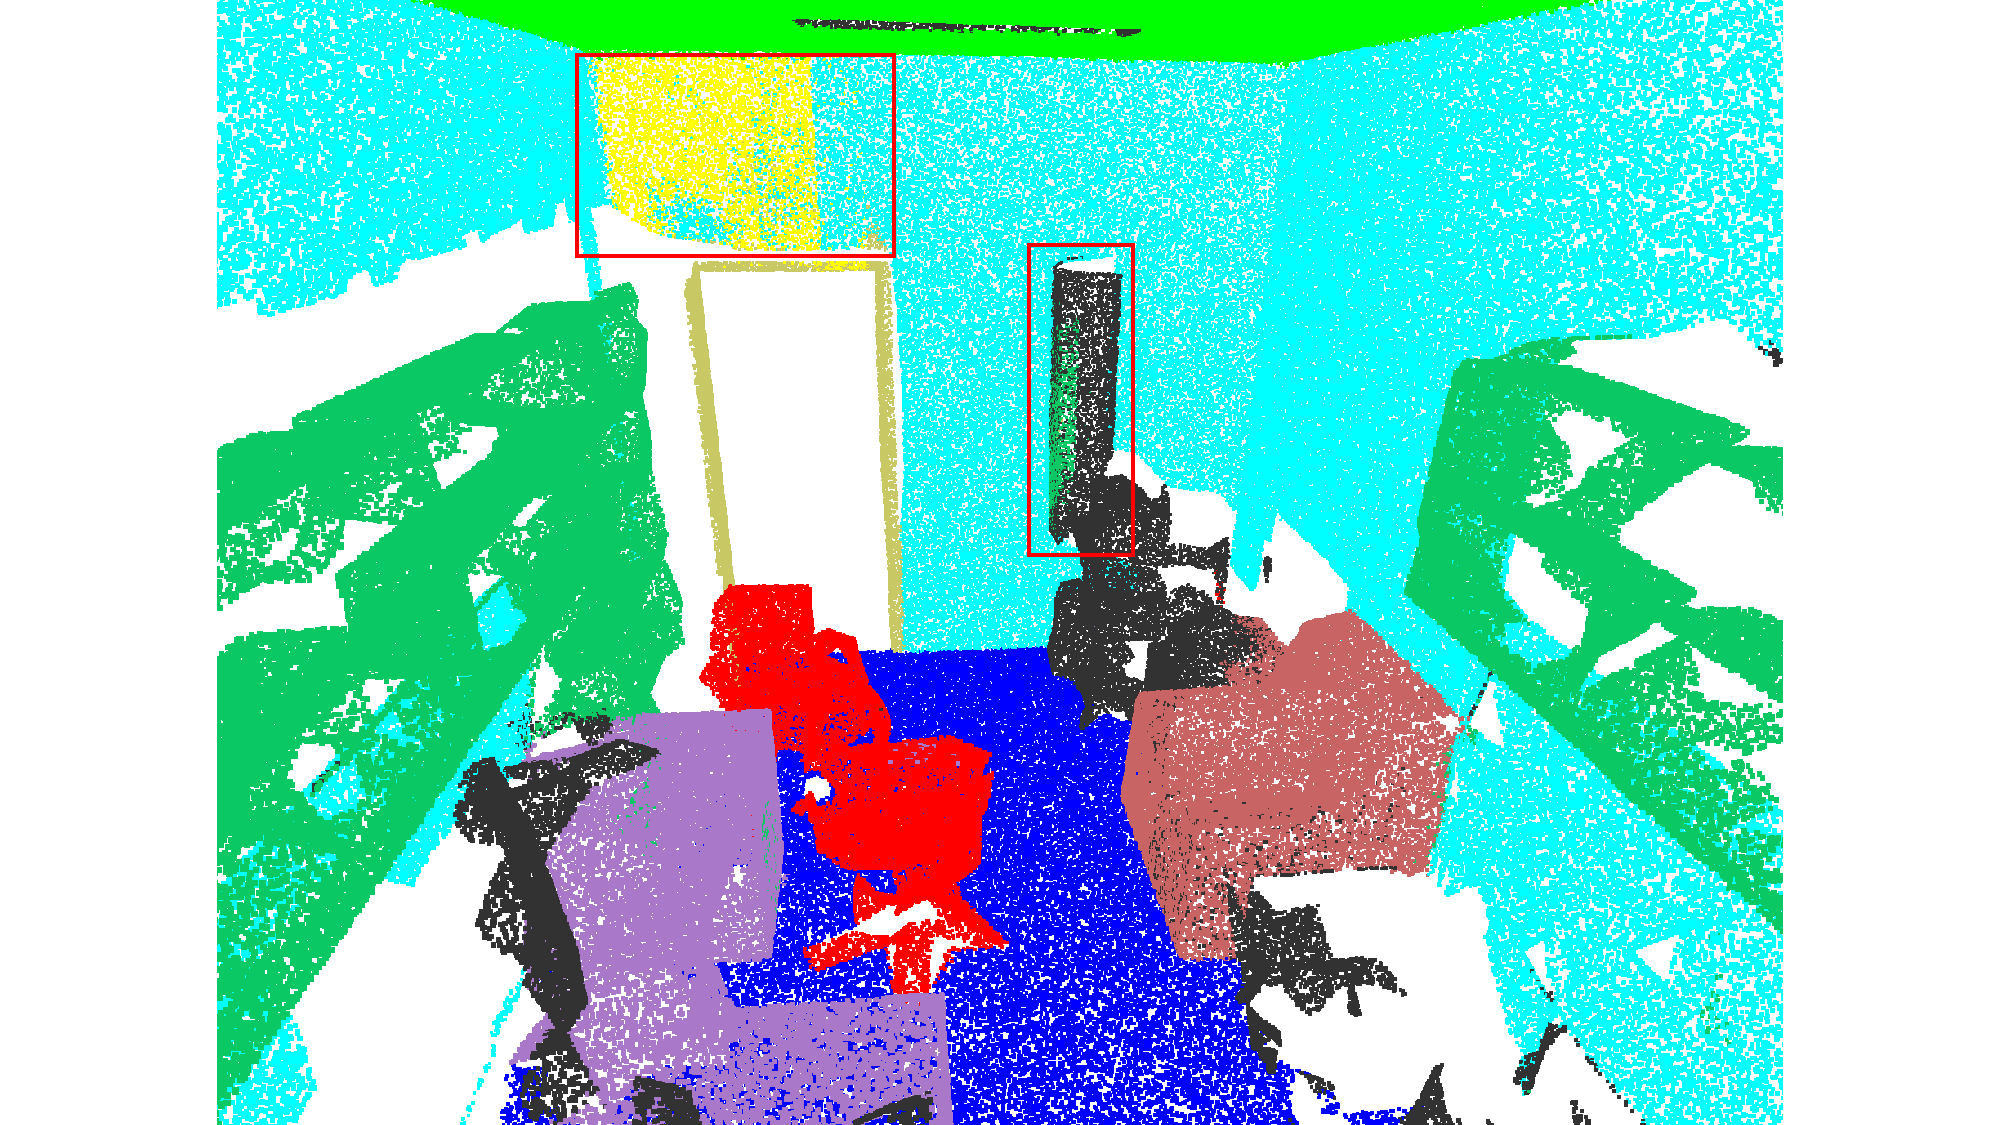
\includegraphics[width=\textwidth]{fig/supplement/semantic_segmentation/office_9/DAPT_office_9.pdf}
    \end{minipage}
    \hfill
    \begin{minipage}{0.185\textwidth}
        \centering
        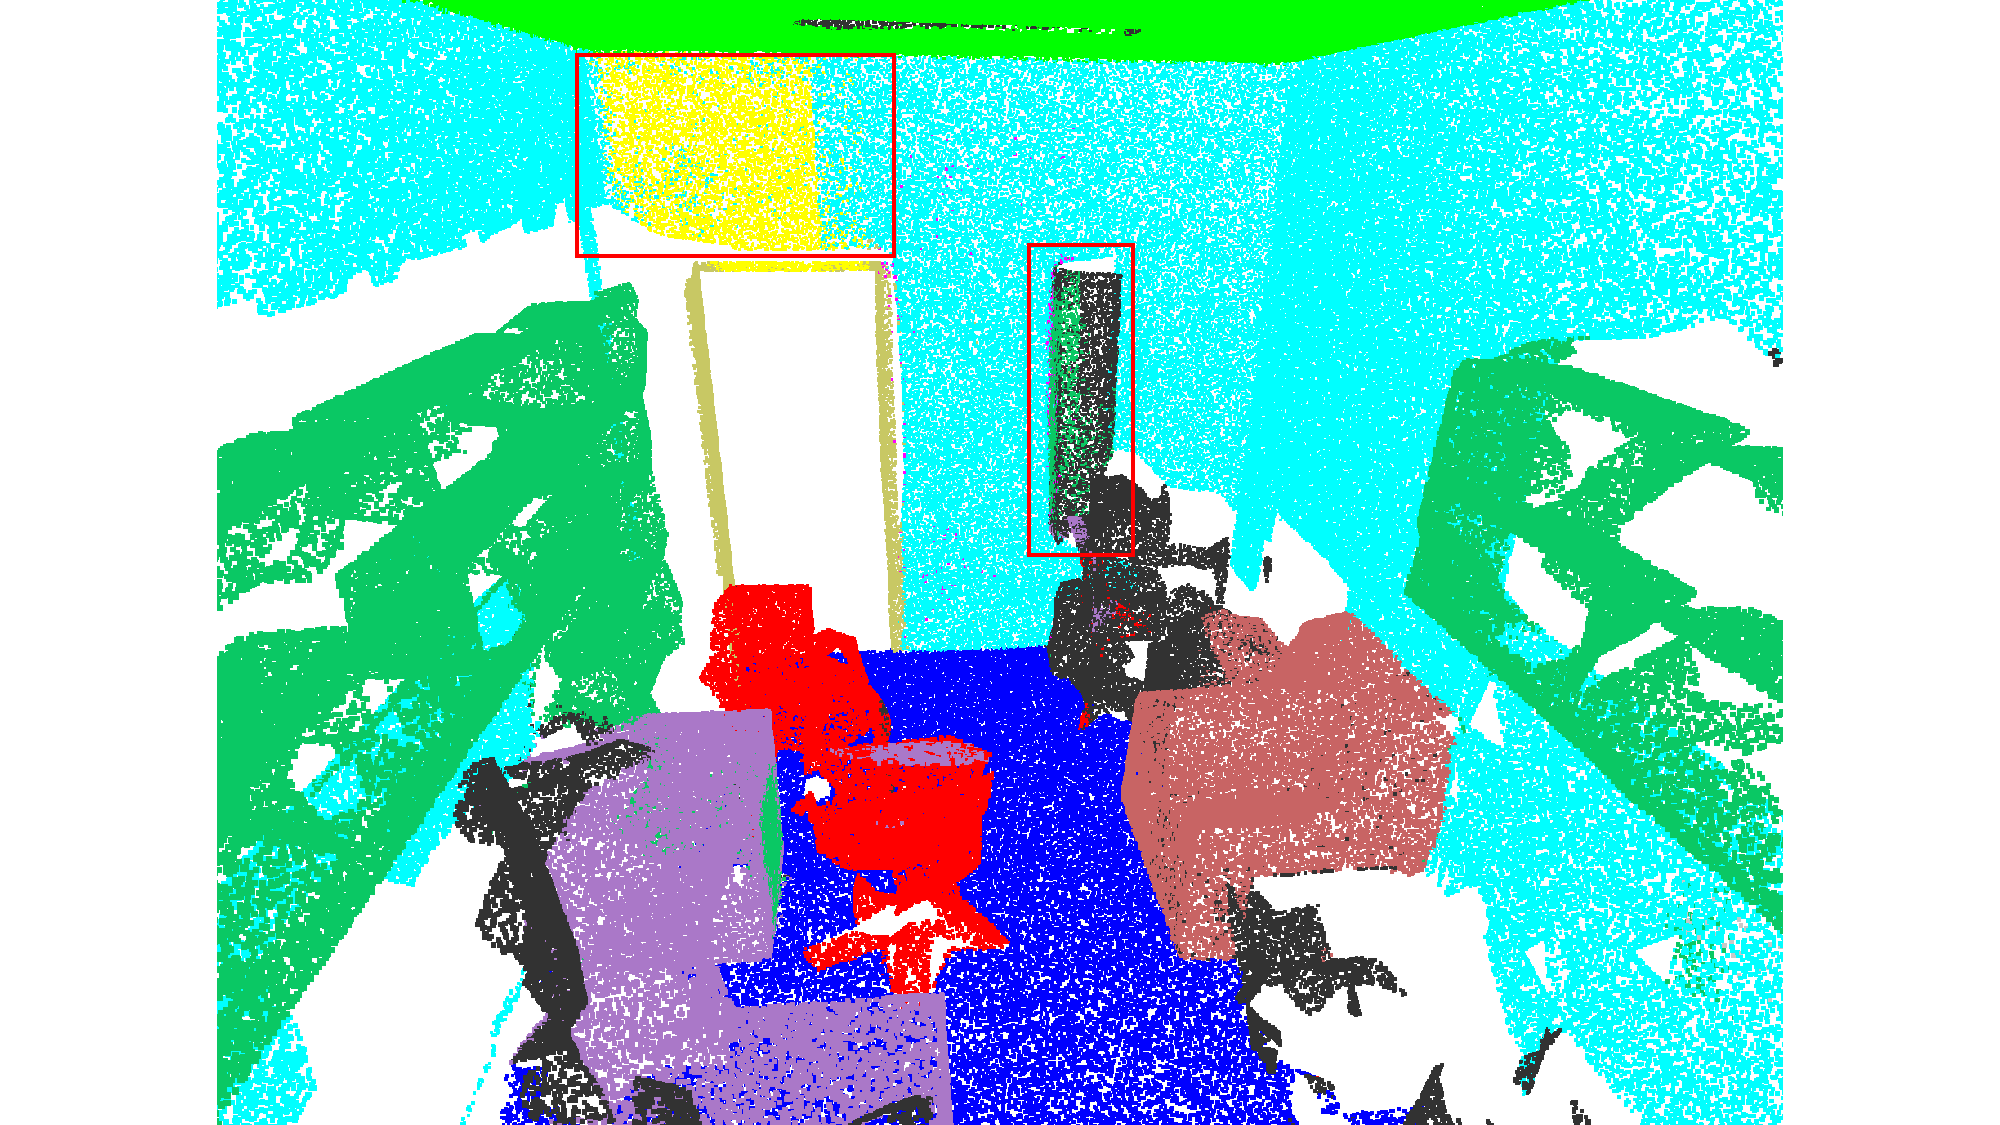
\includegraphics[width=\textwidth]{fig/supplement/semantic_segmentation/office_9/IDPT_office_9.pdf} % 替换为你的图片路径
    \end{minipage}
    \hfill
    \begin{minipage}{0.185\textwidth}
        \centering
        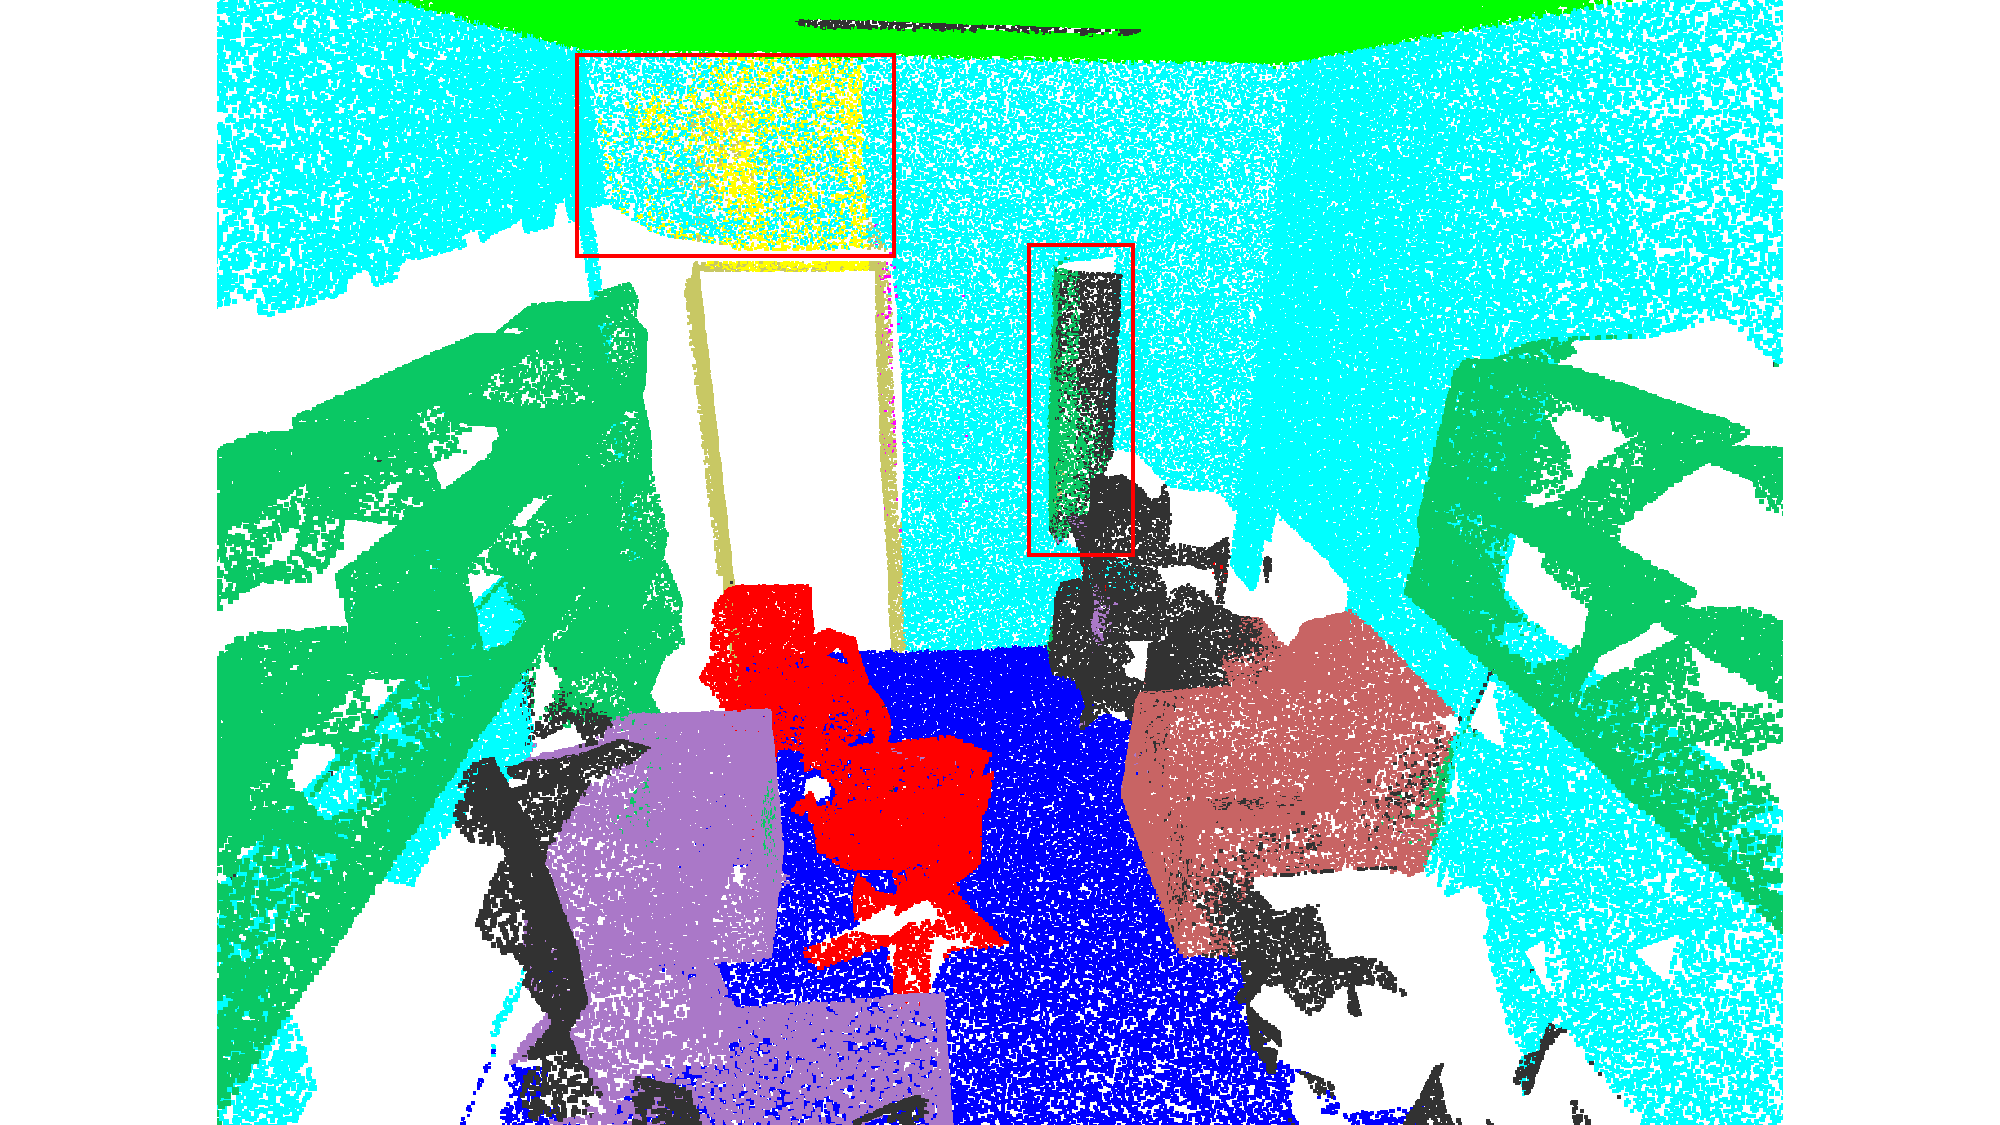
\includegraphics[width=\textwidth]{fig/supplement/semantic_segmentation/office_9/PointGST_office_9.pdf}
    \end{minipage}
    \hfill
    \begin{minipage}{0.185\textwidth}
        \centering
        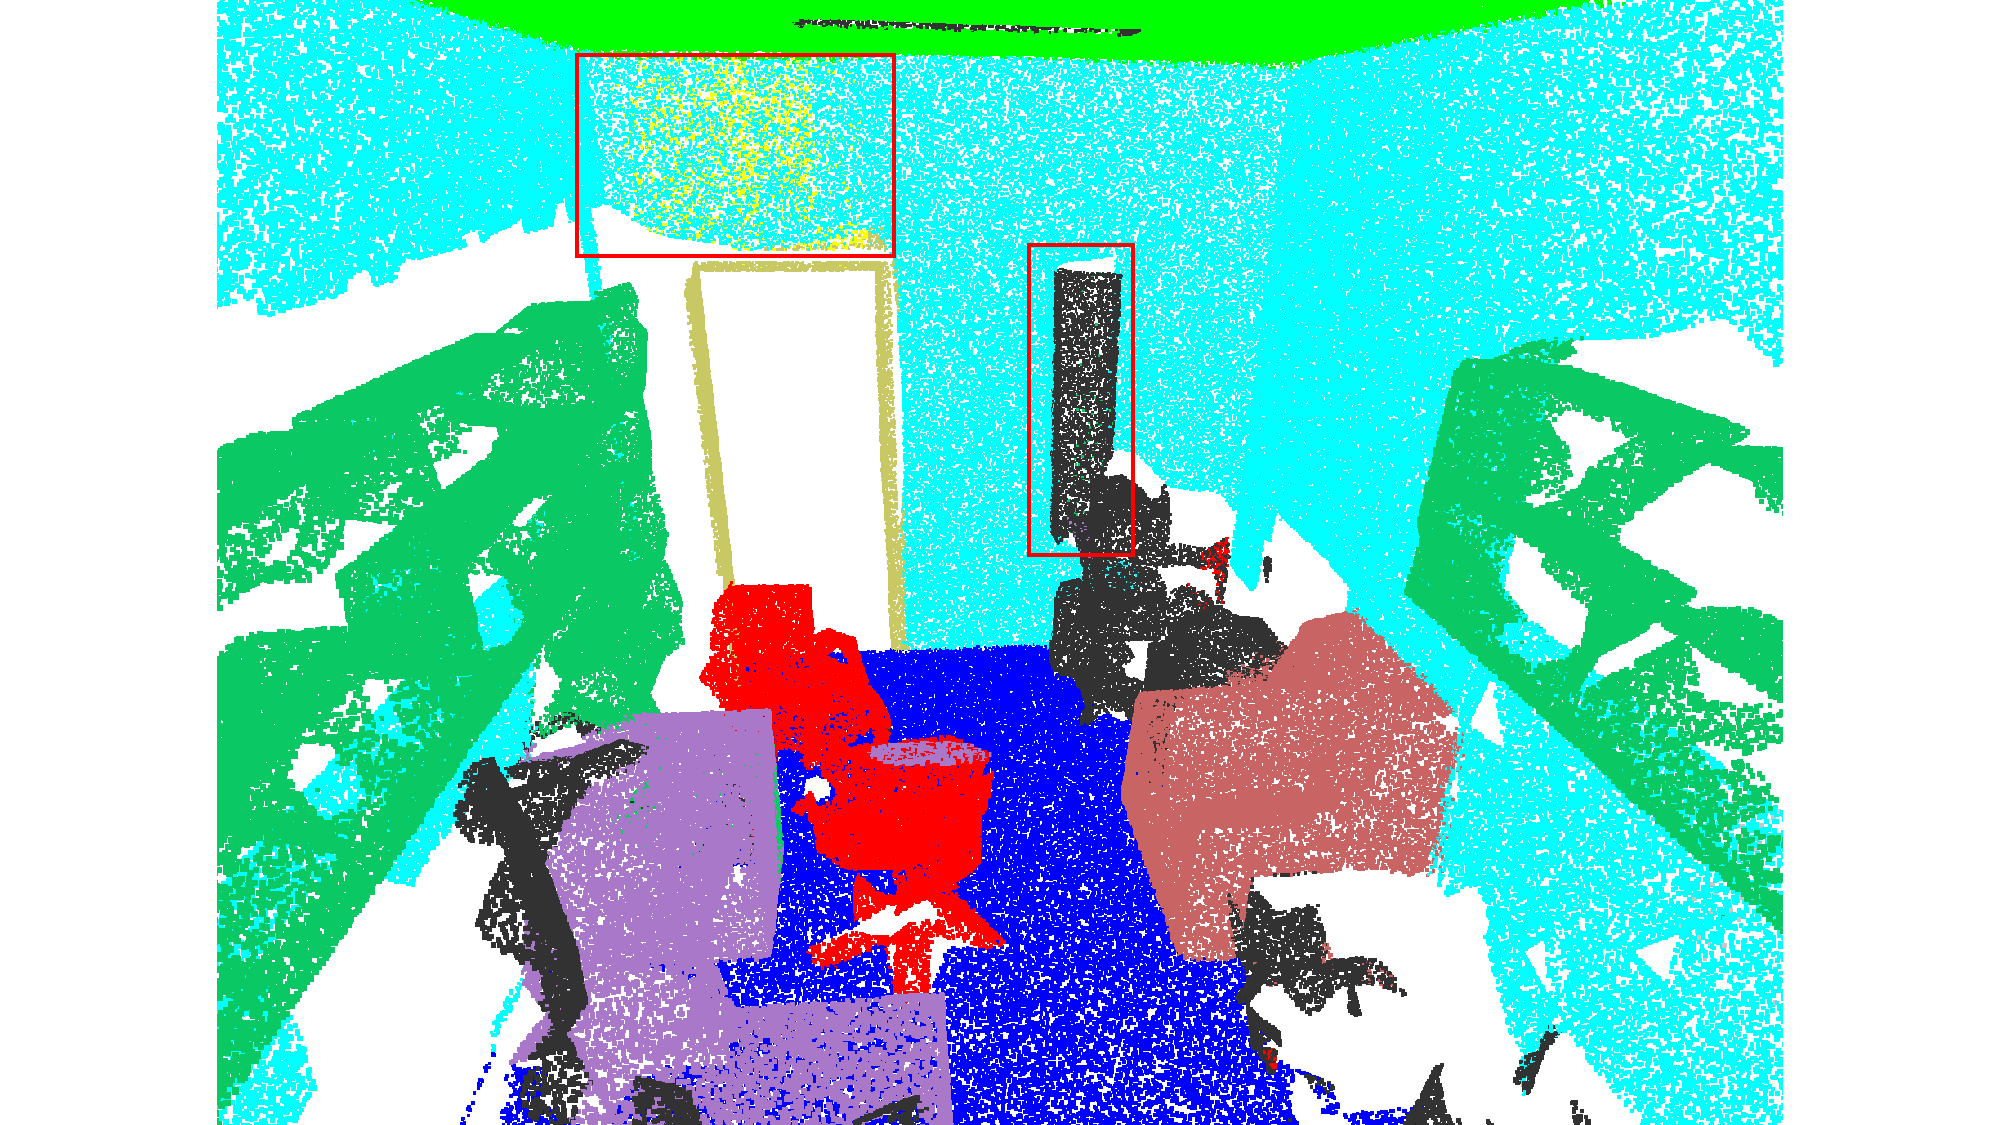
\includegraphics[width=\textwidth]{fig/supplement/semantic_segmentation/office_9/PLT_office_9.pdf}
    \end{minipage}
    \hfill
    \begin{minipage}{0.185\textwidth}
        \centering
        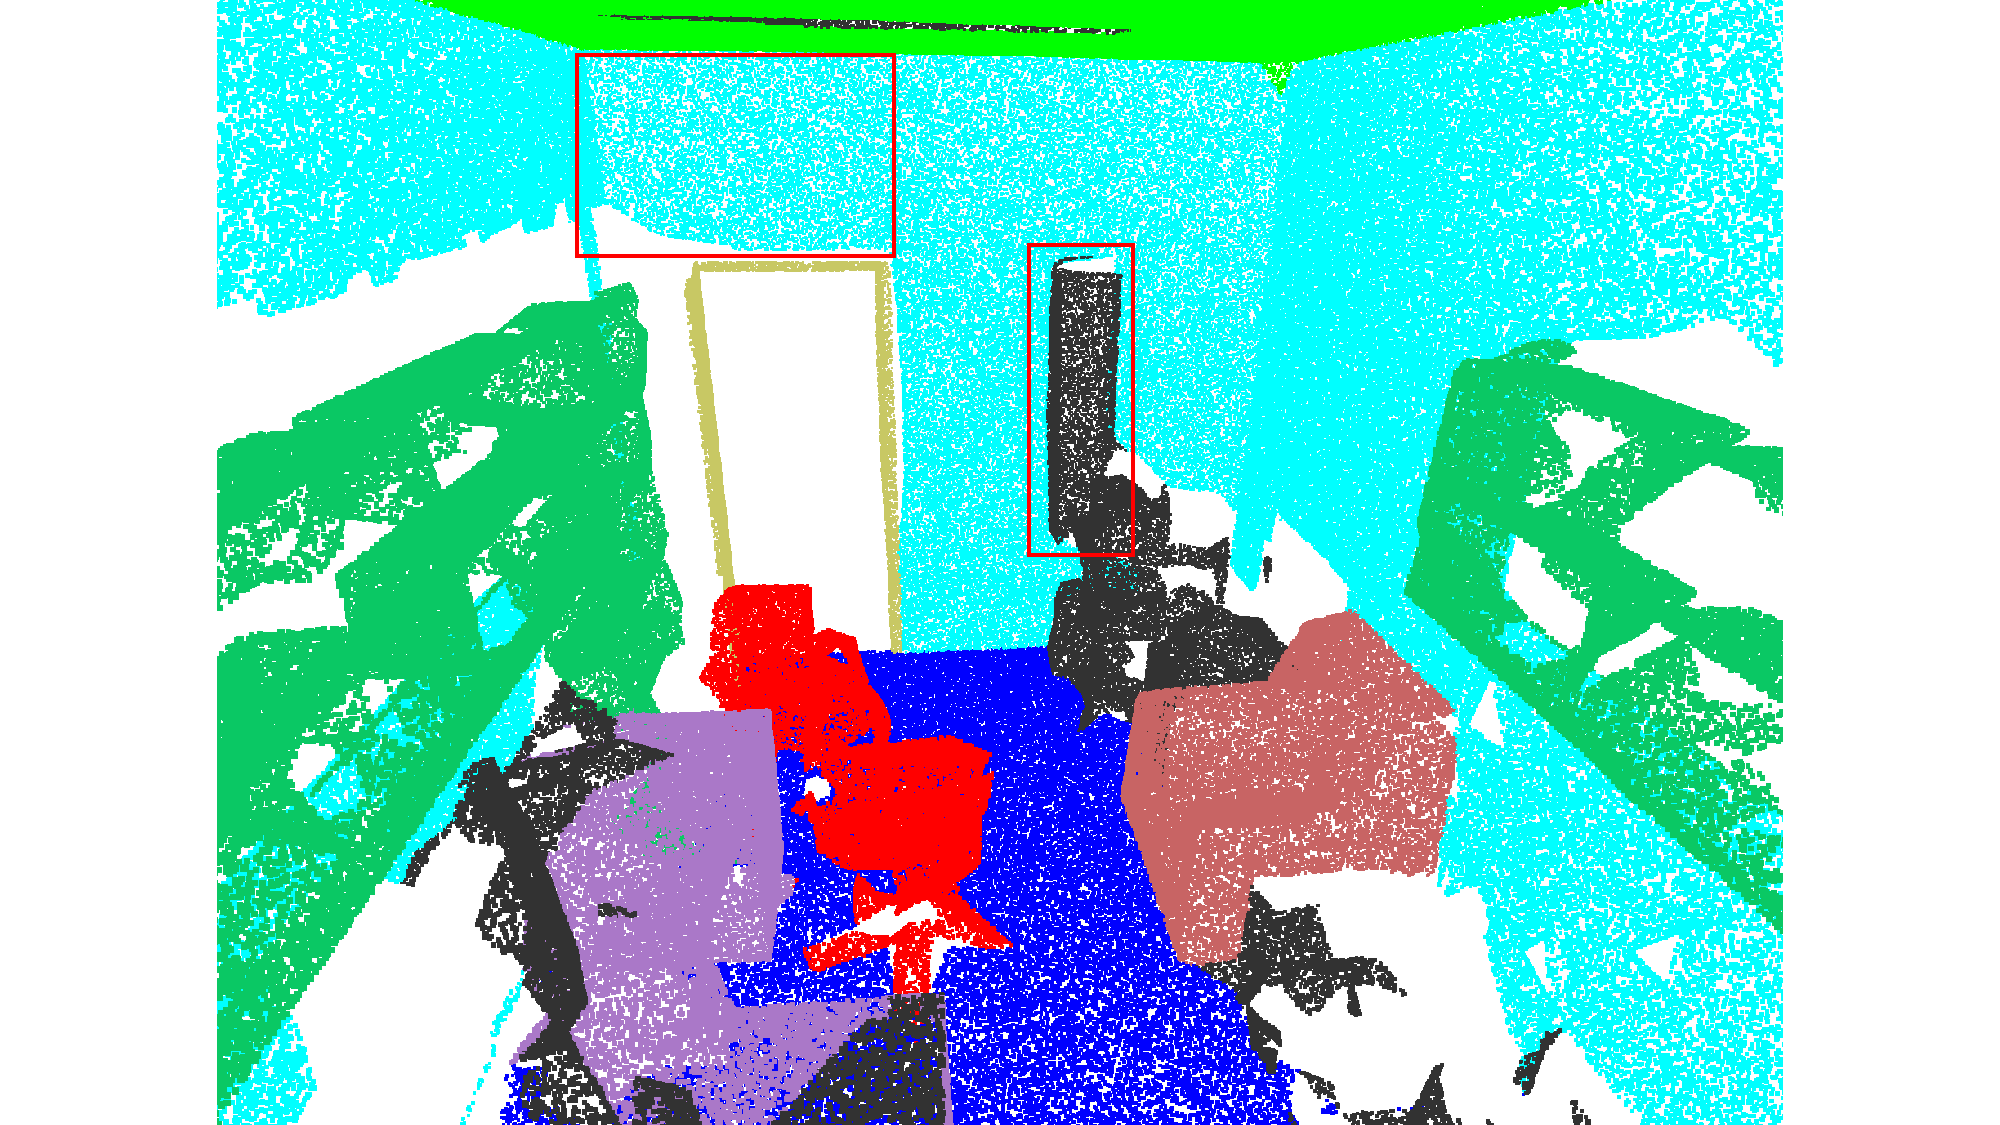
\includegraphics[width=\textwidth]{fig/supplement/semantic_segmentation/office_9/GT_office_9.pdf}
    \end{minipage}
    \hfill

    \vspace{0.5em}

    % 第一行左侧的竖排标签
    \begin{minipage}{0.02\textwidth}
        \centering
        \rotatebox{90}{wc\_2}
    \end{minipage}
    \hfill
    % 第一行图片
    \begin{minipage}{0.185\textwidth}
        \centering
        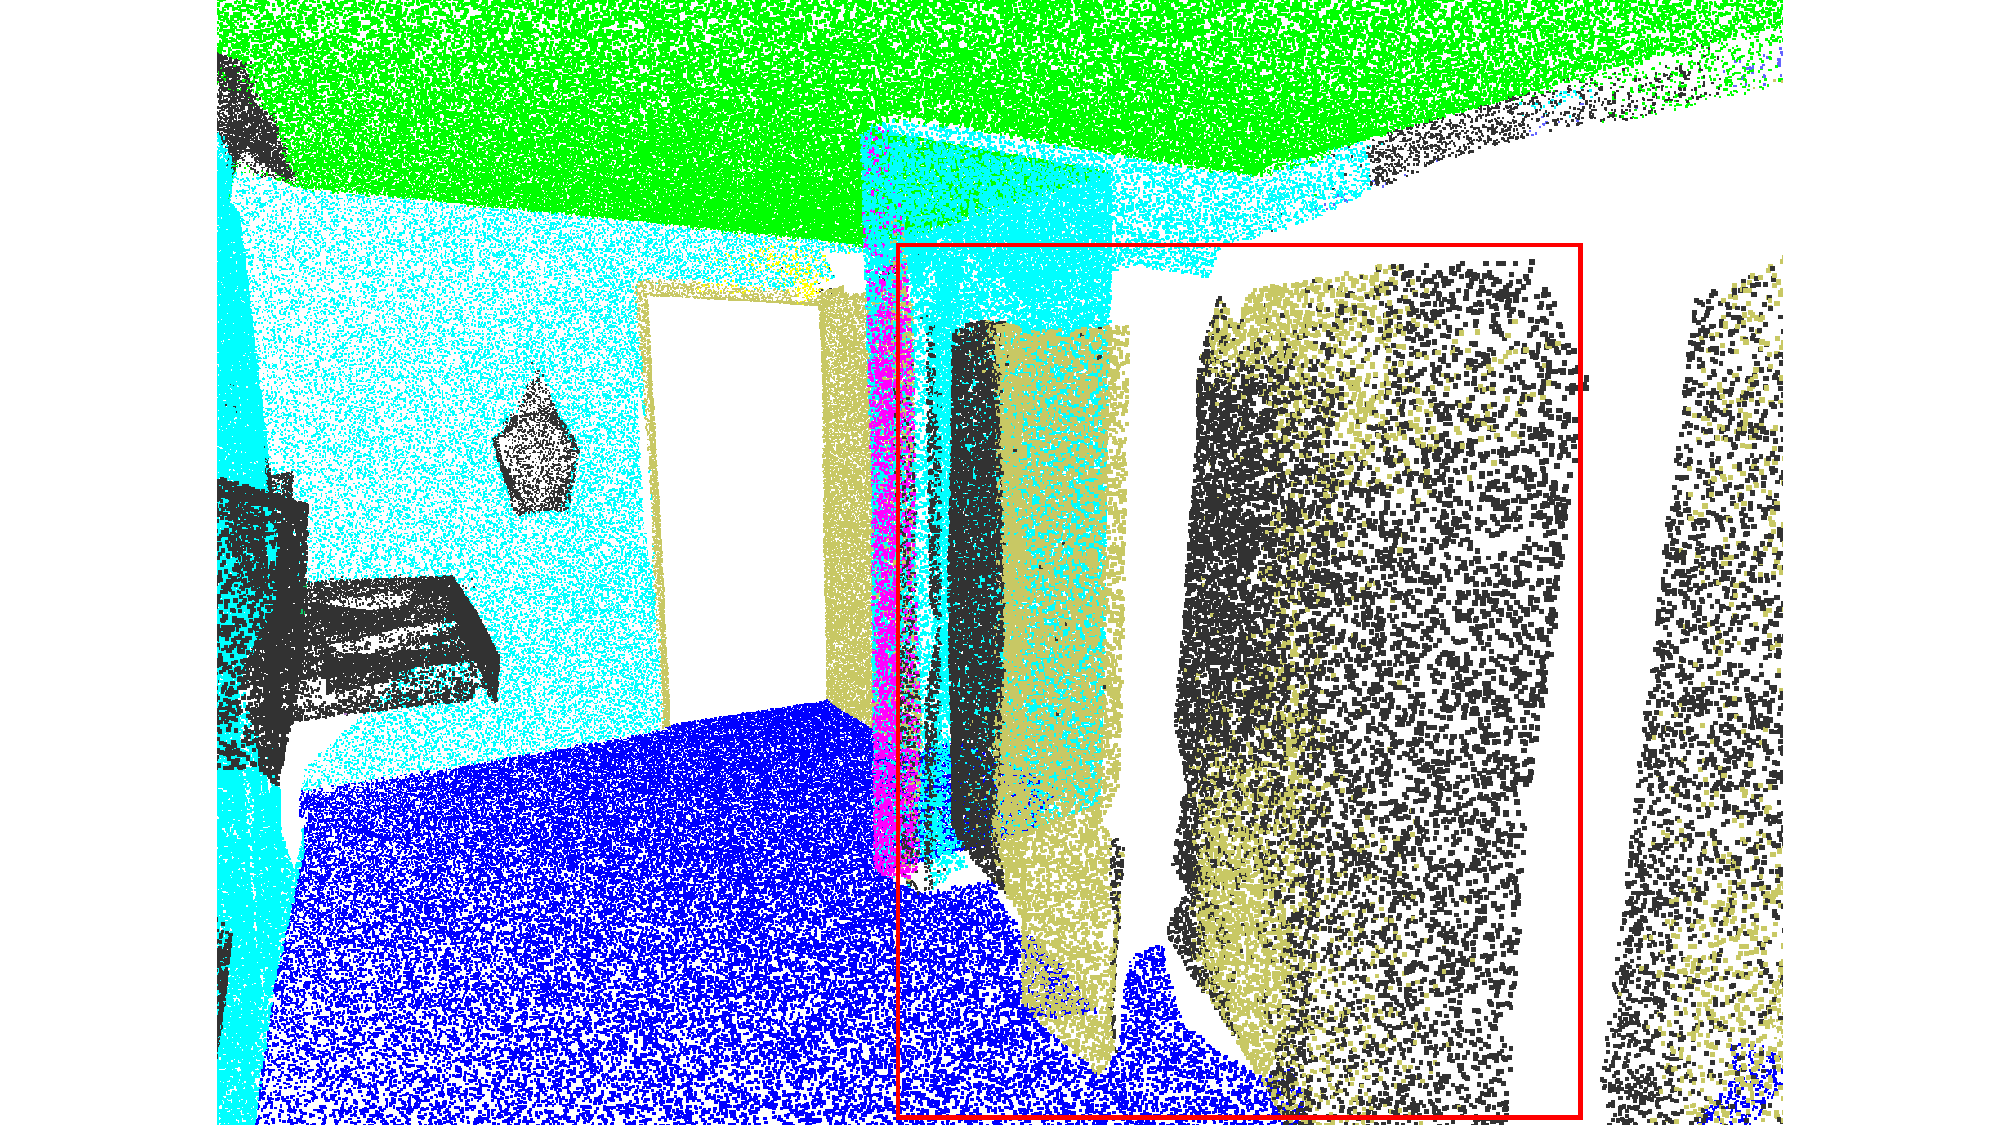
\includegraphics[width=\textwidth]{fig/supplement/semantic_segmentation/wc_2/DAPT_wc_2.pdf}
    \end{minipage}
    \hfill
    \begin{minipage}{0.185\textwidth}
        \centering
        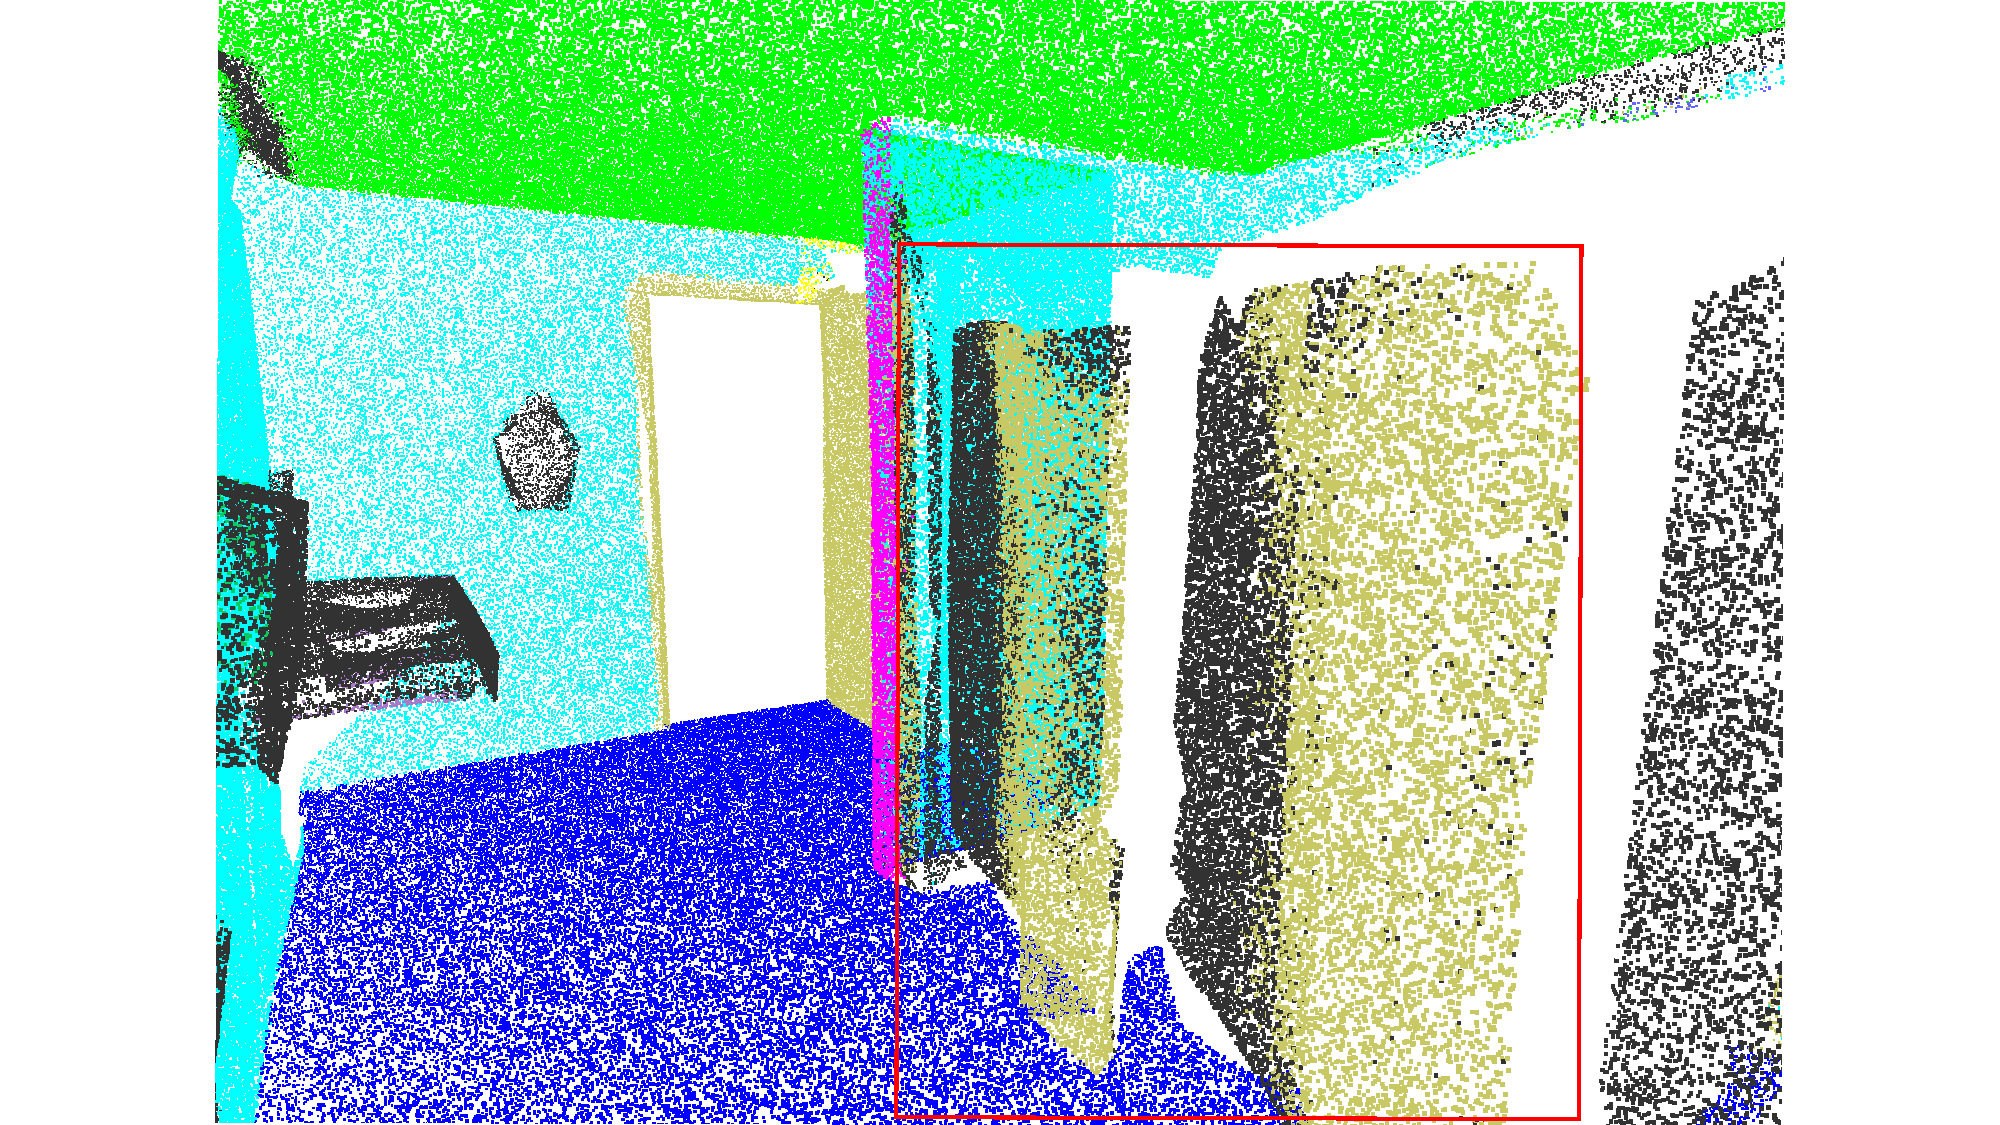
\includegraphics[width=\textwidth]{fig/supplement/semantic_segmentation/wc_2/IDPT_wc_2.pdf} % 替换为你的图片路径
    \end{minipage}
    \hfill
    \begin{minipage}{0.185\textwidth}
        \centering
        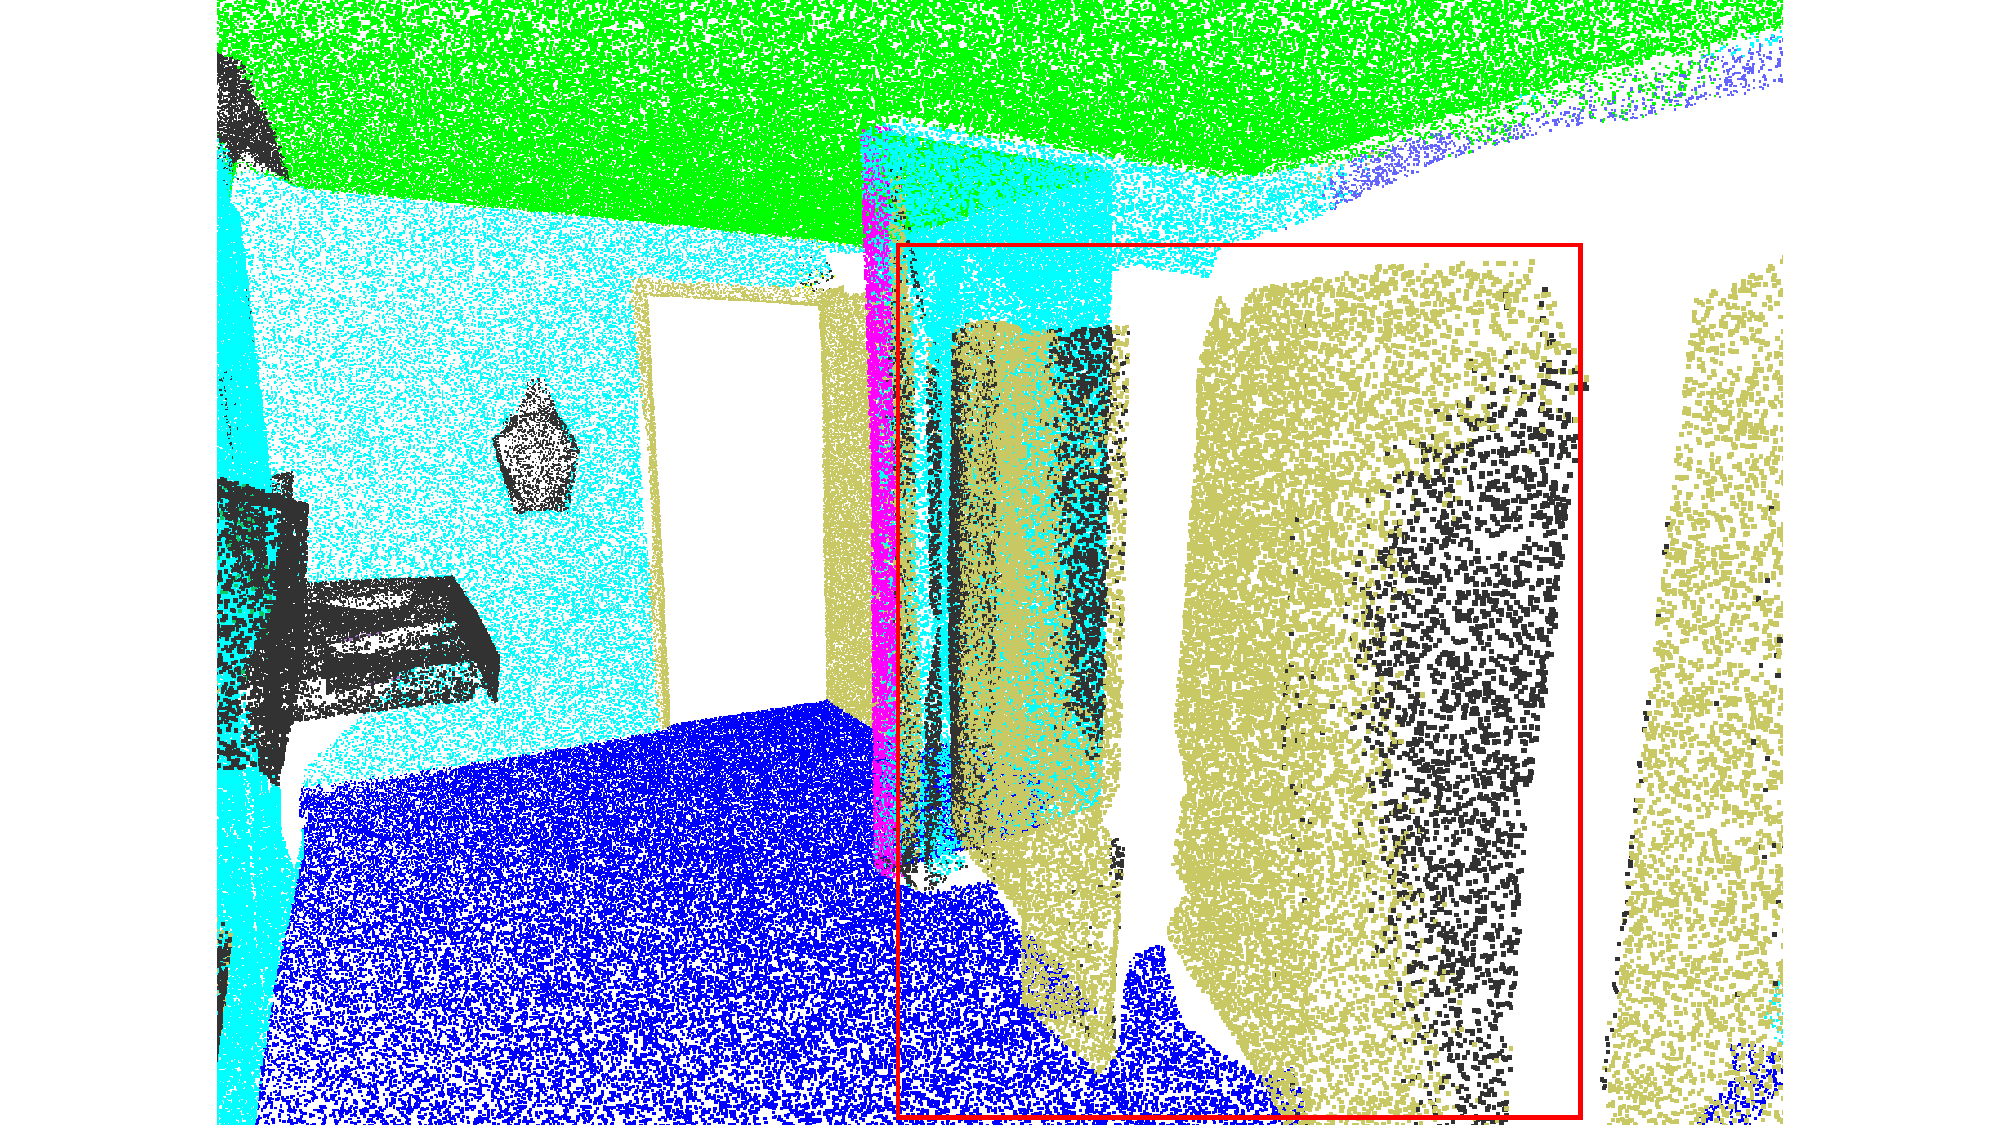
\includegraphics[width=\textwidth]{fig/supplement/semantic_segmentation/wc_2/PointGST_wc_2.pdf}
    \end{minipage}
    \hfill
    \begin{minipage}{0.185\textwidth}
        \centering
        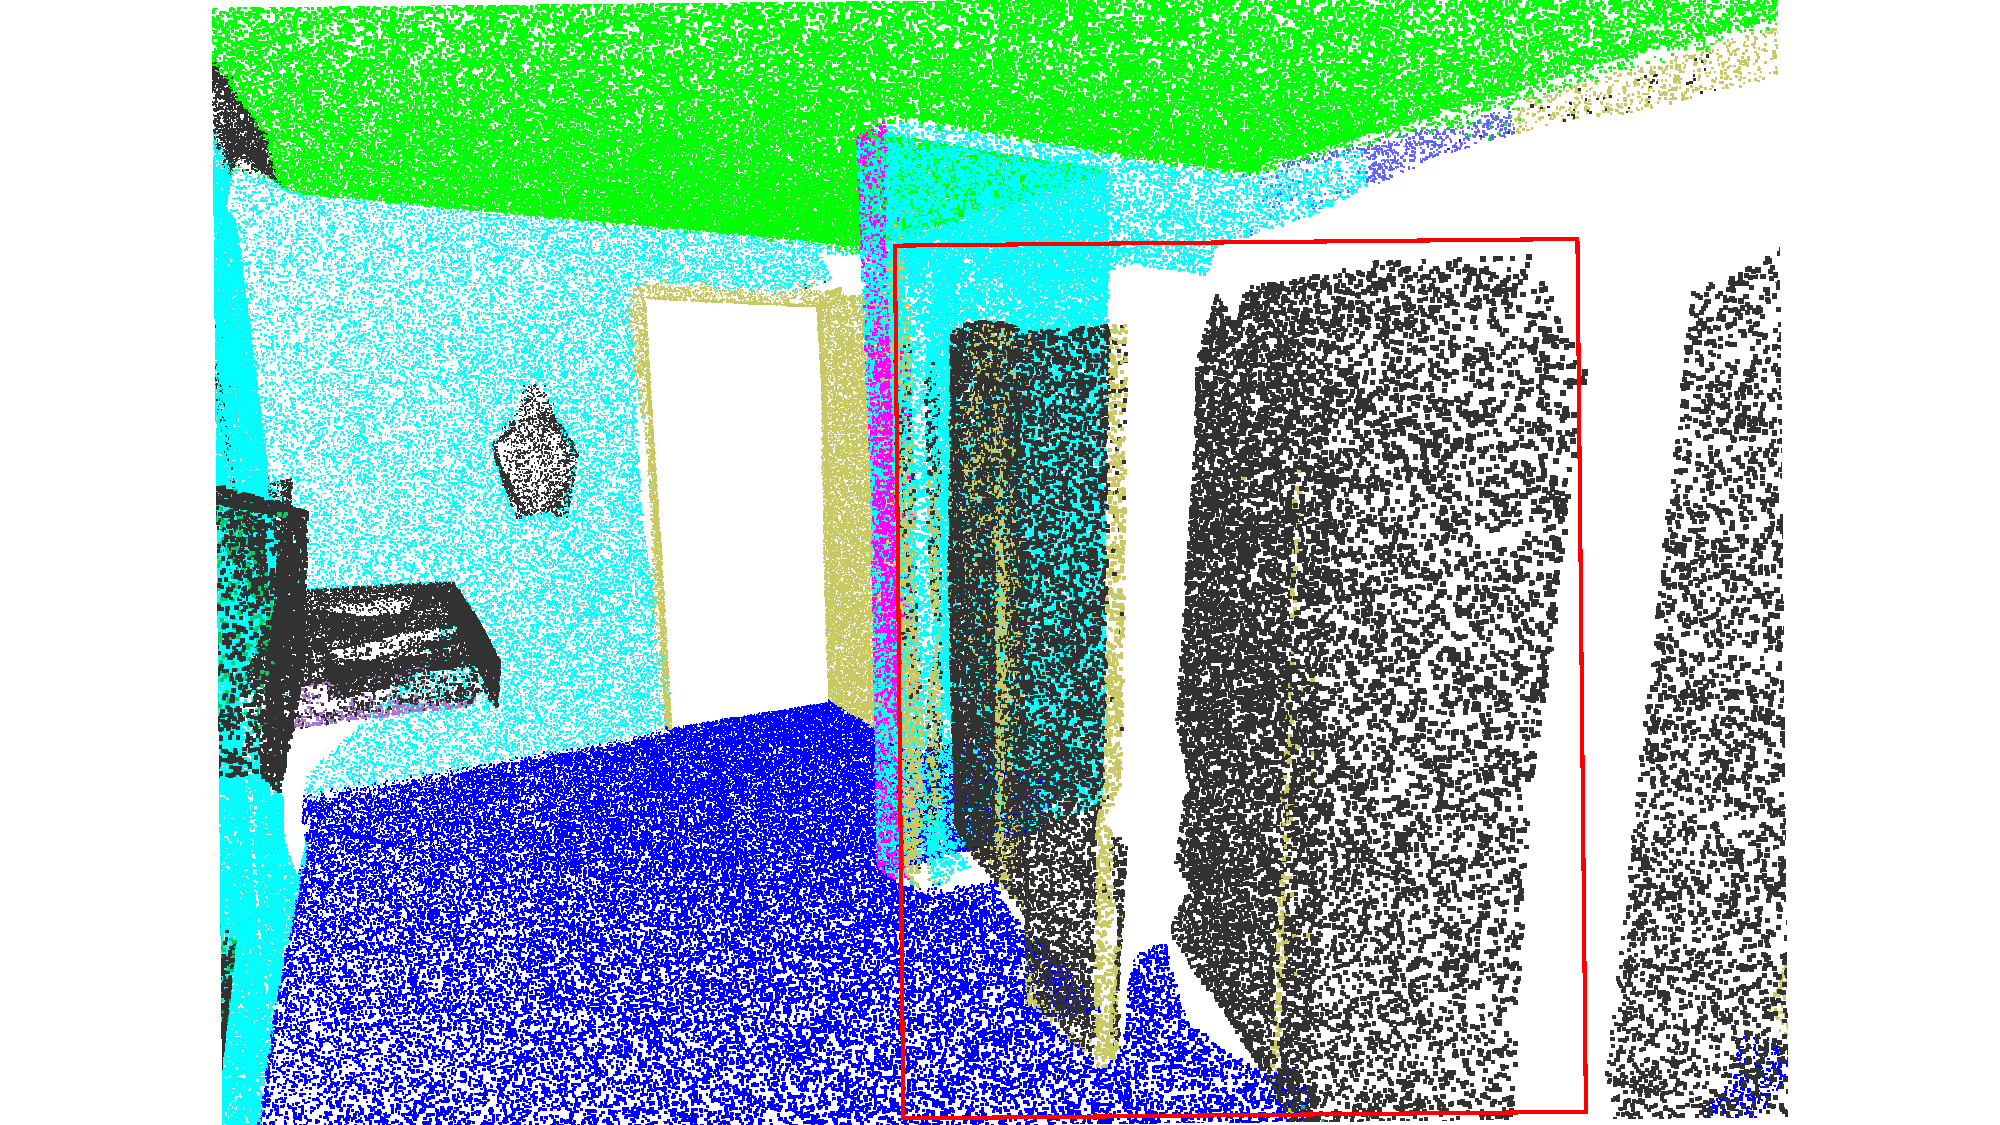
\includegraphics[width=\textwidth]{fig/supplement/semantic_segmentation/wc_2/PLT_wc_2.pdf}
    \end{minipage}
    \hfill
    \begin{minipage}{0.185\textwidth}
        \centering
        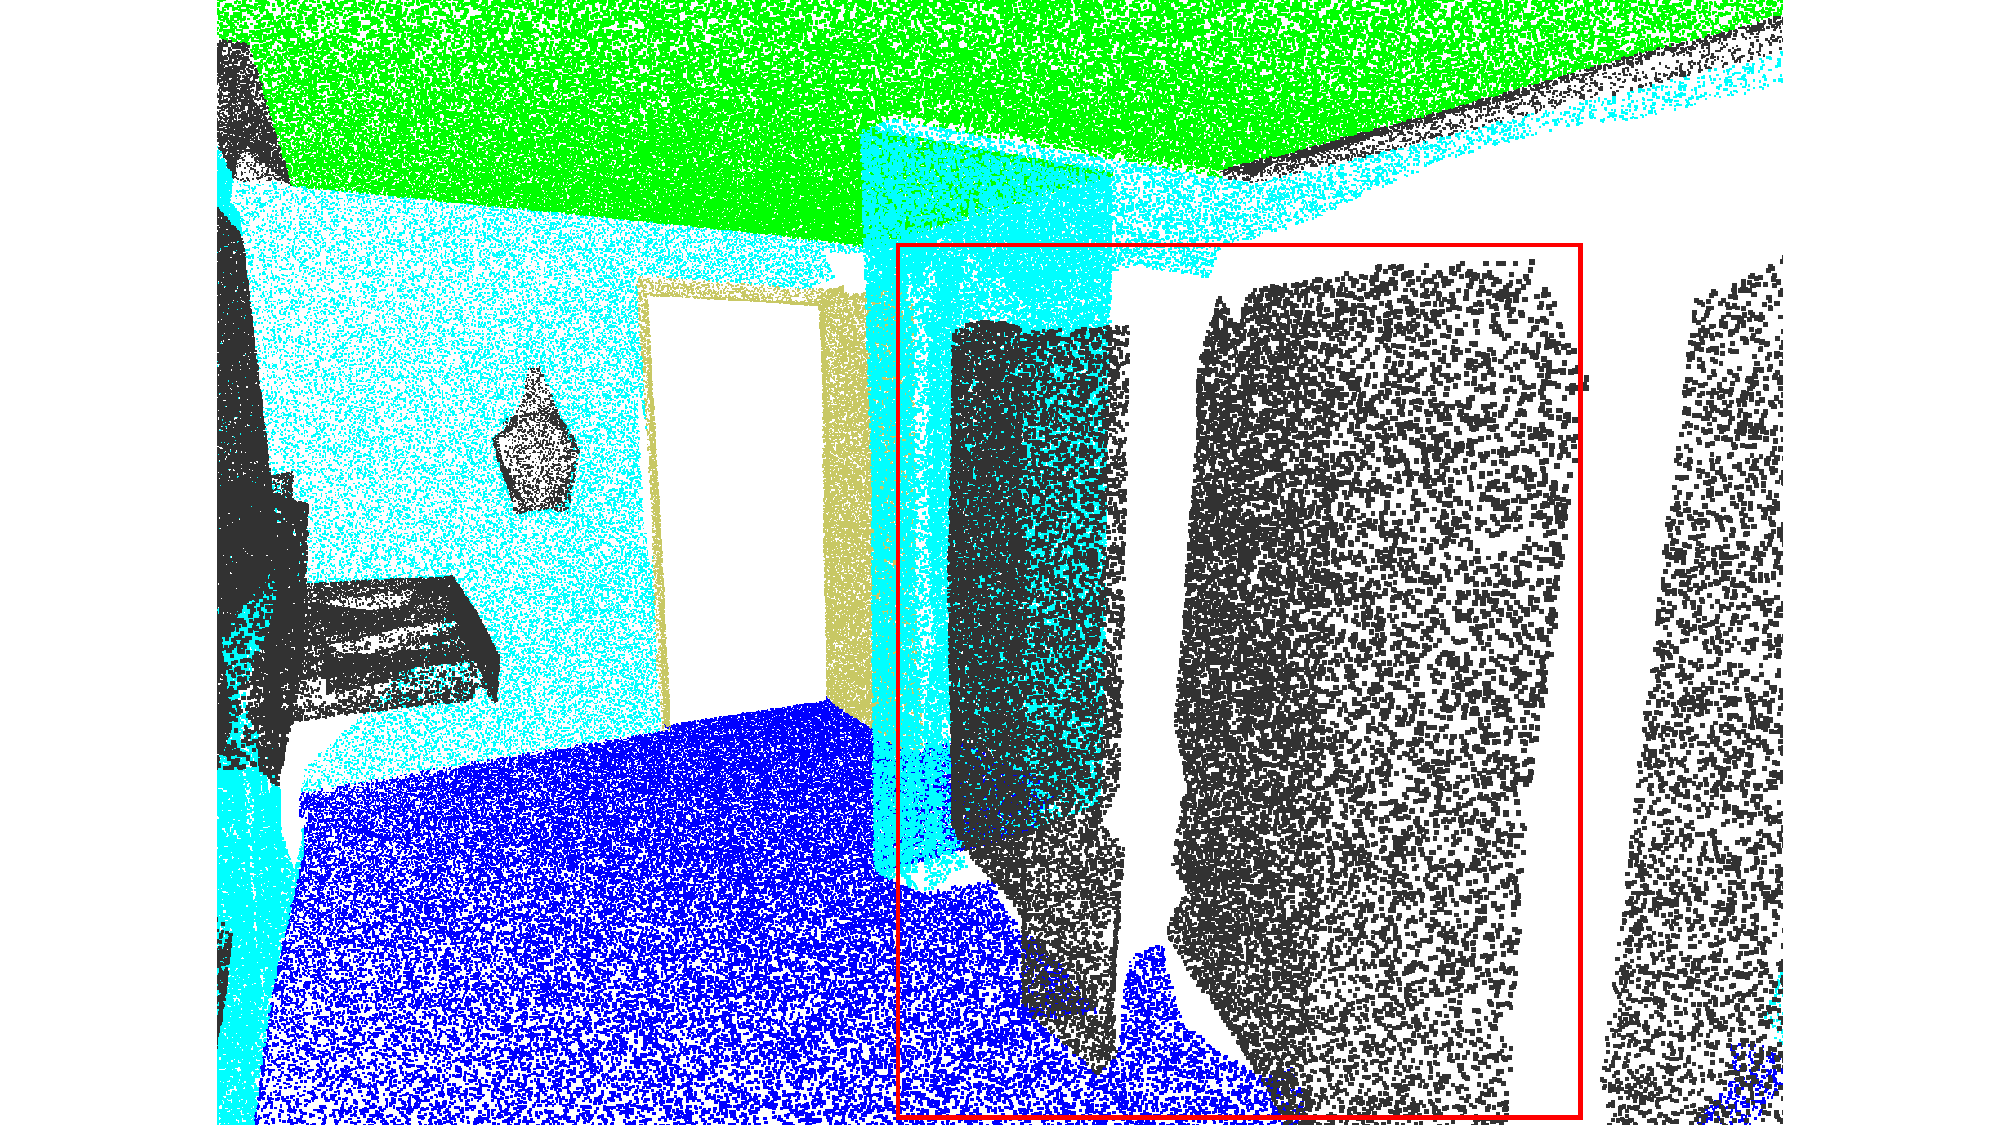
\includegraphics[width=\textwidth]{fig/supplement/semantic_segmentation/wc_2/GT_wc_2.pdf}
    \end{minipage}
    \hfill
    
    %下方的标签
    \vspace{0.5em}
    \begin{minipage}{0.02\textwidth} % 左侧空白区域
        \color{white}{12}
    \end{minipage}
    \hfill
    \begin{minipage}{0.185\textwidth} % 第1列标题
        \centering
        DAPT
    \end{minipage}
    \hfill
    \begin{minipage}{0.185\textwidth} % 第2列标题
        \centering
        IDPT
    \end{minipage}
    \hfill
    \begin{minipage}{0.185\textwidth} % 第3列标题
        \centering
        PointGST
    \end{minipage}
    \hfill
    \begin{minipage}{0.185\textwidth} % 第4列标题
        \centering
        PLT (Ours)
    \end{minipage}
    \hfill
    \begin{minipage}{0.185\textwidth} % 第5列标题
        \centering
        GT
    \end{minipage}
    \hfill
    \caption{The visualization of qualitative results for point cloud semantic segmentation on Area 5 of the S3DIS dataset~\cite{armeni20163d}. %We compare our PLT with previous methods on Area 5 of the S3DIS dataset~\cite{armeni20163d}.
    }
    \label{fig:s3dis_1}

\end{figure*}
